\documentclass[aspectratio=169]{beamer}

\usepackage{graphicx}
\usepackage{amsmath}
\usepackage{amssymb}
\usepackage{geometry}
\usepackage{tikz}

\usepackage{lmodern}
\usepackage{xcolor}

\setlength {\marginparwidth }{2cm}
\usepackage{todonotes}
\presetkeys{todonotes}{inline}{}

\usetheme{singapore}

\setbeamercovered{transparent}

\newcommand{\shellcmd}[1]{~\\ \indent\indent\texttt{\textcolor{teal}{ \$ #1}\\}}

\title{Version control \& git}
\subtitle{An indroduction}
\date{LISCO Lab Meeting. \today}

% https://ubucon.de/files/Git-Workshop.pdf

\begin{document}

\maketitle

\section{Indroduction}

%%%%%%%%%%%%%%%%%%%%%%%%%%%%%%%%%%%%%%%%%%%%%%%%%%

\begin{frame}
\frametitle{What is version control?}

\begin{itemize}
	\item Manage versions of files projects etc...
\end{itemize}

\end{frame}

%%%%%%%%%%%%%%%%%%%%%%%%%%%%%%%%%%%%%%%%%%%%%%%%%%

\begin{frame}
\frametitle{What can be versioned?}

\begin{itemize}
	\item source code
	\item images
	\item music
	\item etc...
\end{itemize}
$\rightarrow$ anything
\end{frame}

%%%%%%%%%%%%%%%%%%%%%%%%%%%%%%%%%%%%%%%%%%%%%%%%%%

\begin{frame}
\frametitle{Why version control?}

\begin{itemize}
	\item Traceability
	\item "Jump" between different versions
	\item Team work and collaboration
\end{itemize}
\vspace{.5cm}
Changes are saved with:
\begin{itemize}
	\item Author
	\item Date and time
	\item Change note
\end{itemize}

\end{frame}

%%%%%%%%%%%%%%%%%%%%%%%%%%%%%%%%%%%%%%%%%%%%%%%%%%

\begin{frame}
\frametitle{Why version control?}

\begin{center}
	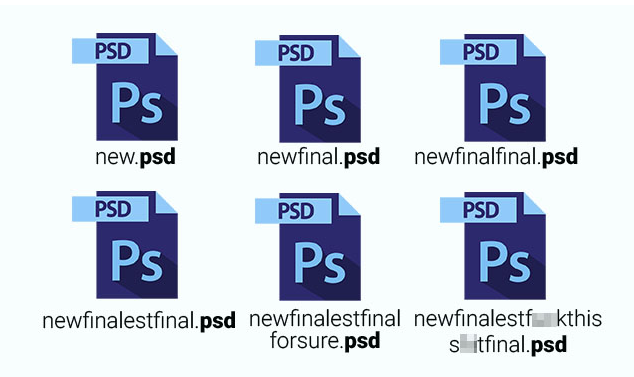
\includegraphics[width=10cm]{graphics/psdversions.png}
\end{center}

\end{frame}

%%%%%%%%%%%%%%%%%%%%%%%%%%%%%%%%%%%%%%%%%%%%%%%%%%

\begin{frame}
\frametitle{Three kinds of version control}

\todo{Maybe remove this slide? Maybe reduce?}

\begin{columns}[T]
	\begin{column}{0.3\textwidth}
		\begin{block}{Local}
			\uncover<2-4>{
				\begin{itemize}
					\item Only on local machine
					\item for working alone on a project
					\item No data security
				\end{itemize}
			}
		\end{block}
	\end{column}
	\begin{column}{0.3\textwidth}
		\begin{block}{Centralized}
			\uncover<3-4>{
				\begin{itemize}
					\item Repository is on remote server
					\item working copy on client
					\item any change on repository happens online
				\end{itemize}
			}
		\end{block}
	\end{column}
	\begin{column}{0.4\textwidth}
		\begin{block}{Distributed}
			\uncover<4>{
				\begin{itemize}
					\item Complete clone on client AND server
					\item only necessary network traffic
					\item high data security through redundancy
				\end{itemize}
			}
		\end{block}
	\end{column}

\end{columns}


\end{frame}



\section{Get Started}
%%%%%%%%%%%%%%%%%%%%%%%%%%%%%%%%%%%%%%%%%%%%%%%%%%

\begin{frame}
\frametitle{Configure git}

\shellcmd{git config (--global) user.name "Felix Nonnengiesser"}
\shellcmd{git config (--global) user.email s8819853@stud.uni-frankfurt.de}

\end{frame}

%%%%%%%%%%%%%%%%%%%%%%%%%%%%%%%%%%%%%%%%%%%%%%%%%%

\begin{frame}
\frametitle{Initialize a repository}


\begin{block}{Create a project folder:}<1-2>
	\shellcmd{mkdir website-with-git}
	\shellcmd{cd website-with-git}
\end{block}

\begin{block}{Initialize repository:}<2>
	
	\shellcmd{git init}

	\texttt{Initialized empty Git repository in C:/Users/Felix/website-with-git/.git/}
\end{block}


\end{frame}

%%%%%%%%%%%%%%%%%%%%%%%%%%%%%%%%%%%%%%%%%%%%%%%%%%

\begin{frame}
\frametitle{Initialize a repository}
\shellcmd{ls -l .git}
~\\
\texttt{total 7\\
	-rw-r--r-- 1 Felix 197121 130 Aug 27 12:02 config \\
	-rw-r--r-- 1 Felix 197121  73 Aug 27 12:02 description\\
	-rw-r--r-- 1 Felix 197121  23 Aug 27 12:02 HEAD\\
	drwxr-xr-x 1 Felix 197121   0 Aug 27 12:02 hooks/\\
	drwxr-xr-x 1 Felix 197121   0 Aug 27 12:02 info/\\
	drwxr-xr-x 1 Felix 197121   0 Aug 27 12:02 objects/\\
	drwxr-xr-x 1 Felix 197121   0 Aug 27 12:02 refs/\\
}
\end{frame}

%%%%%%%%%%%%%%%%%%%%%%%%%%%%%%%%%%%%%%%%%%%%%%%%%%

\begin{frame}
\frametitle{git status}

\shellcmd{git status}
~\\
\texttt{On branch master\\
No commits yet\\
nothing to commit (create/copy files and use "git add" to track)
}

\end{frame}

%%%%%%%%%%%%%%%%%%%%%%%%%%%%%%%%%%%%%%%%%%%%%%%%%%

\begin{frame}
\frametitle{Preperations for our little project}
\todo{add link to project files. Or clone git repo?}
Download template from
\texttt{http://template.zip}
\\~\\
For Linux users:
\shellcmd{wget http://template.zip}
\end{frame}

%%%%%%%%%%%%%%%%%%%%%%%%%%%%%%%%%%%%%%%%%%%%%%%%%%

\begin{frame}
\frametitle{git status}
\todo{update outputs with new project files}
\shellcmd{git status}
\texttt{On branch master\\
	Untracked files:\\
	(use "git add <file>..." to include in what will be committed)\\
	~\\
	\hspace{1cm}\textcolor{red}{myprofile.html}\\
	~\\
	nothing added to commit but untracked files present (use "git add" to track)}

\end{frame}

%%%%%%%%%%%%%%%%%%%%%%%%%%%%%%%%%%%%%%%%%%%%%%%%%%

\begin{frame}
\frametitle{git add}

\shellcmd{git add \textcolor{red}{myprofile.html}}
~\\
\shellcmd{git status}
\texttt{On branch master\\
	Changes to be committed:\\
	(use "git reset HEAD <file>..." to unstage)\\
	~\\
	\hspace{1cm}\textcolor{green}{new file:   myprofile.html}
}
\end{frame}

%%%%%%%%%%%%%%%%%%%%%%%%%%%%%%%%%%%%%%%%%%%%%%%%%%

\begin{frame}
\frametitle{git commit}
\shellcmd{git commit -m "added profile page"}
\texttt{[master c18ea18] added profile page\\
	1 file changed, 36 insertions(+)\\
	create mode 100644 myprofile.html
}
\end{frame}

%%%%%%%%%%%%%%%%%%%%%%%%%%%%%%%%%%%%%%%%%%%%%%%%%%

\begin{frame}
\frametitle{git status}
\todo{update outputs with new project files}
\shellcmd{git status}
\texttt{On branch master\\
	nothing to commit, working tree clean
}
\end{frame}

%%%%%%%%%%%%%%%%%%%%%%%%%%%%%%%%%%%%%%%%%%%%%%%%%%

\begin{frame}
\frametitle{git log}
\shellcmd{git log}
\texttt{Author: Felix <nonni1997@hotmail.de>\\
	Date:~~ Tue Aug 27 16:04:27 2019 +0200\\
	~\\
	\hspace{1cm}added profile page	
}
\end{frame}

%%%%%%%%%%%%%%%%%%%%%%%%%%%%%%%%%%%%%%%%%%%%%%%%%%

\begin{frame}
\frametitle{Change content}

\begin{columns}[T]
	\begin{column}{0.6\textwidth}
		\begin{block}{}<1-2>
			\begin{itemize}
				\item Open the \textcolor{red}{myprofile.html} file with a text editor of your choice. e.g. notepad++
				\item Fill in the gaps
			\end{itemize}
		\end{block}
		\begin{block}{}<2>
			\begin{figure}
				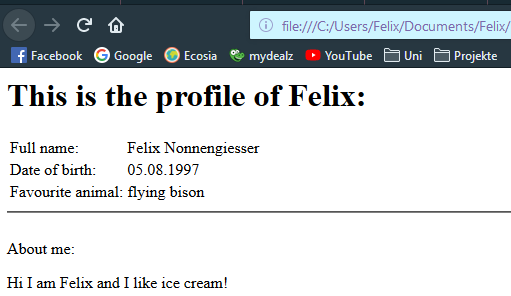
\includegraphics[width= 0.8\textwidth]{graphics/profile.png}
			\end{figure}
		\end{block}
	\end{column}
	\begin{column}{0.4\textwidth}
		\begin{block}{}<1-2>
			\begin{figure}
				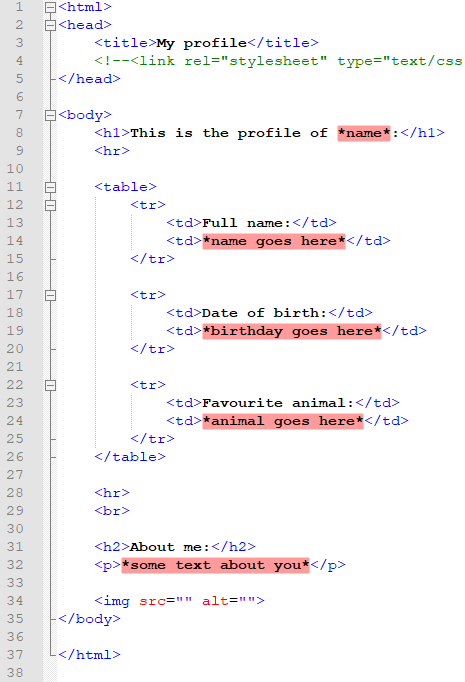
\includegraphics[height=0.8\textheight]{graphics/profile_edit.png}
			\end{figure}
			
		\end{block}
	\end{column}
\end{columns}


\end{frame}

%%%%%%%%%%%%%%%%%%%%%%%%%%%%%%%%%%%%%%%%%%%%%%%%%%

\begin{frame}
\frametitle{git add \& git commit}

\shellcmd{git add myprofile.html}
\shellcmd{git commit -m "updated profile information"}
\texttt{[master 7de6662] updated profile information\\
	1 file changed, 5 insertions(+), 5 deletions(-)
}

\end{frame}

%%%%%%%%%%%%%%%%%%%%%%%%%%%%%%%%%%%%%%%%%%%%%%%%%%

\begin{frame}
\frametitle{git log}
\shellcmd{git log}
\texttt{\textcolor{orange}{commit 7de6662d0efd82b3e469594be85d38561c3fc536 (HEAD -> master)}\\
	Author: Felix <nonni1997@hotmail.de>\\
	Date:   Tue Aug 27 16:44:47 2019 +0200\\
	~\\
	updated profile information\\
	~\\
	\textcolor{orange}{commit c18ea185996a38679a0f3a623a9c10459045dccc}\\
	Author: Felix <nonni1997@hotmail.de>\\
	Date:   Tue Aug 27 16:04:27 2019 +0200\\
	~\\
	added profile page
}
\end{frame}

%%%%%%%%%%%%%%%%%%%%%%%%%%%%%%%%%%%%%%%%%%%%%%%%%%

\begin{frame}
\frametitle{Change content}
\end{frame}

%%%%%%%%%%%%%%%%%%%%%%%%%%%%%%%%%%%%%%%%%%%%%%%%%%

\begin{frame}
\frametitle{git status}
\end{frame}

%%%%%%%%%%%%%%%%%%%%%%%%%%%%%%%%%%%%%%%%%%%%%%%%%%

\begin{frame}
\frametitle{git diff}
\end{frame}

%%%%%%%%%%%%%%%%%%%%%%%%%%%%%%%%%%%%%%%%%%%%%%%%%%

\section{Branching}

\begin{frame}
\frametitle{Branching}
\centering
\begin{figure}
	
\includegraphics[width=4cm]{graphics/git_logo.png}
	\caption{Git logo}
\end{figure}

\end{frame}

%%%%%%%%%%%%%%%%%%%%%%%%%%%%%%%%%%%%%%%%%%%%%%%%%%

\begin{frame}
\frametitle{Why branching}
\begin{itemize}
	\item stable
	\item development
	\item newAwesomeFeature
	\item featureXY
\end{itemize}
\end{frame}

%%%%%%%%%%%%%%%%%%%%%%%%%%%%%%%%%%%%%%%%%%%%%%%%%%

\begin{frame}
\frametitle{Add a new Feature}
Let's add an image of ourselves to the profile page!
\vspace{0.5cm}
\begin{itemize}
	\item we want to add a new feature
	\item we don't want to have unfinished features in our main/master branch
	\item we want to tinker around without breaking the master
\end{itemize}
\vspace{0.5cm}
$\rightarrow$ We create a new branch!
\end{frame}

%%%%%%%%%%%%%%%%%%%%%%%%%%%%%%%%%%%%%%%%%%%%%%%%%%

\begin{frame}
\frametitle{Show existing branches}
\shellcmd{git branch}
\texttt{* master}
\end{frame}

%%%%%%%%%%%%%%%%%%%%%%%%%%%%%%%%%%%%%%%%%%%%%%%%%%

\begin{frame}
\frametitle{Create a new branch}
\shellcmd{git branch picture}
~\\
\shellcmd{git branch}
\texttt{* master \\ ~~picture}

\end{frame}

%%%%%%%%%%%%%%%%%%%%%%%%%%%%%%%%%%%%%%%%%%%%%%%%%%

\begin{frame}
\frametitle{Change branch}
\shellcmd{git checkout picture}
\texttt{Switched to branch 'picture'}
~\\
\shellcmd{git branch}
\texttt{~~master\\ * picture
}
\end{frame}

%%%%%%%%%%%%%%%%%%%%%%%%%%%%%%%%%%%%%%%%%%%%%%%%%%

\begin{frame}
\frametitle{Implement our new feature}
	\begin{columns}[T]
		\todo{tidy up}
		\begin{column}{0.7\textwidth}
				\begin{itemize}
					\item open the html file
					\item remove the comment tags \texttt{\textcolor{green}{<!--}} and \texttt{\textcolor{green}{-->}} in line \todo{add line number} XX 
					\item replace \textcolor{blue}{"url.to.img"} with the URL to your chosen image
				\end{itemize}
				\vspace{.5cm}
				\texttt{<img \textcolor{red}{src}=\textcolor{blue}{"url.to.img"} \textcolor{red}{alt}=\textcolor{blue}{"Description"}>}
		\end{column}
		\begin{column}{0.3\textwidth}
				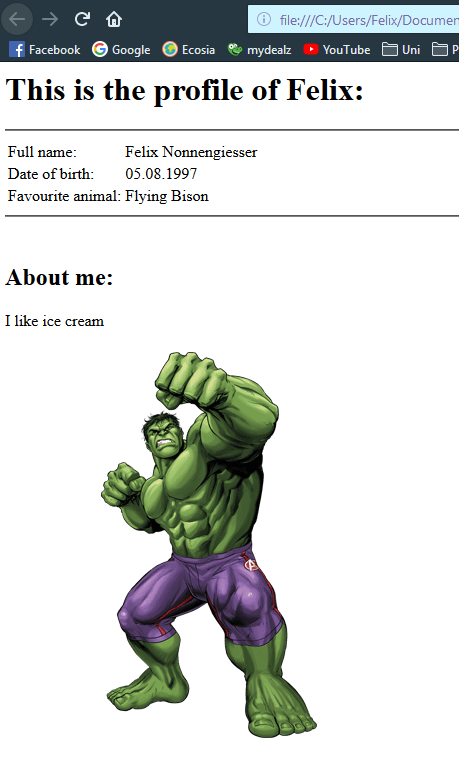
\includegraphics[width=.9\textwidth]{graphics/profile_with_picture.png}
		\end{column}
	\end{columns}
	\todo{change title of page in this branch to provoke merge conflict later}		
\end{frame}

%%%%%%%%%%%%%%%%%%%%%%%%%%%%%%%%%%%%%%%%%%%%%%%%%%

\begin{frame}
\frametitle{Commit changes}
	\shellcmd{git add myprofile.html}
	\shellcmd{git commit -m "add picture to profile page"}
	\todo{add outputs?}
\end{frame}

%%%%%%%%%%%%%%%%%%%%%%%%%%%%%%%%%%%%%%%%%%%%%%%%%%

\begin{frame}
\frametitle{Change branches}
\begin{itemize}
	\item Let's go back to the master branch \shellcmd{git checkout master}
	\item When loading our profile page, our picture is gone 
\end{itemize}
	$\rightarrow$ \textcolor{red}{master} branch is not affected by changes in other branches.\\
	\hspace{.5cm}We will find out later how to add these changes to the master branch.
\end{frame}

%%%%%%%%%%%%%%%%%%%%%%%%%%%%%%%%%%%%%%%%%%%%%%%%%%

\begin{frame}
\frametitle{Another feature}
	Our page looks a bit boring. Let's beautify it!
	\todo{add output}
\begin{itemize}
	\item New feature $\rightarrow$ new branch \shellcmd{git branch style}
	\item Change to new branch \shellcmd{git checkout style}
\end{itemize}
\end{frame}

%%%%%%%%%%%%%%%%%%%%%%%%%%%%%%%%%%%%%%%%%%%%%%%%%%

\begin{frame}
\frametitle{Adding a new file to our repository}
\begin{itemize}
	\item We add a "stylesheet" to our website to make it look better.
	\item Let's add the stylesheet to our git repository \shellcmd{git add styles.css} \todo{add output}
	\item Link the stylesheet to your html page: 
	\begin{itemize}
		\item open the html file in the editor
		\item remove the comment tags \texttt{\textcolor{green}{<!--}} and \texttt{\textcolor{green}{-->}} in line \todo{add line number} XX 
	\end{itemize}
\end{itemize}
Have a look at the new version of the profile page!
\todo{change title of page in this branch to provoke merge conflict later}
\todo {add commit...}
\end{frame}

%%%%%%%%%%%%%%%%%%%%%%%%%%%%%%%%%%%%%%%%%%%%%%%%%%

\begin{frame}
\frametitle{The updated page}
\centering
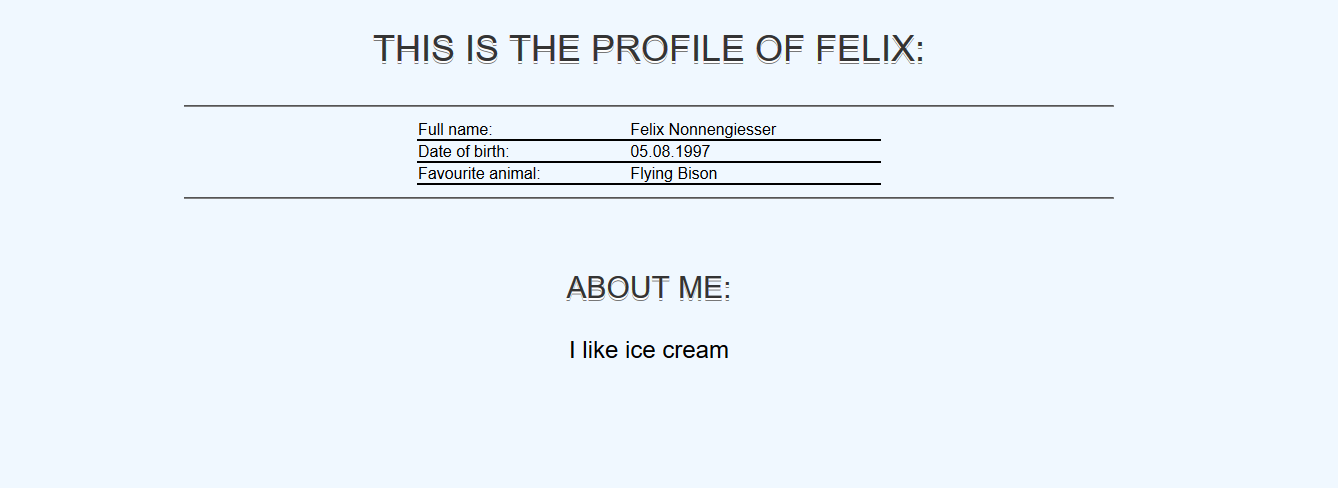
\includegraphics[width=.9\textwidth]{graphics/profile_with_css.png}
\end{frame}

%%%%%%%%%%%%%%%%%%%%%%%%%%%%%%%%%%%%%%%%%%%%%%%%%%

\begin{frame}
\frametitle{Our current status}
\begin{itemize}
	\item We do have three different versions of our website
	\item None of them contains all the features we want
	\item But we want our master branch combining all these features!
\end{itemize}
\end{frame}


%%%%%%%%%%%%%%%%%%%%%%%%%%%%%%%%%%%%%%%%%%%%%%%%%%

\begin{frame}
\frametitle{Merge branches}
\todo{add output}
\begin{itemize}
	\item to merge changes into the master branch we have to be inside the master branch \shellcmd{git checkout master}
	\item \vspace{.5cm}Merge the picture branch into the master: \shellcmd{git merge picture} 
	\item Merge the style branch into the master: \shellcmd{git merge style} 
	\todo{handle merge conflict}
\end{itemize}
\end{frame}

%%%%%%%%%%%%%%%%%%%%%%%%%%%%%%%%%%%%%%%%%%%%%%%%%%

\begin{frame}
\frametitle{Recap: What did we do?}
\todo{add tikz graph with version history}
\end{frame}

%%%%%%%%%%%%%%%%%%%%%%%%%%%%%%%%%%%%%%%%%%%%%%%%%%

\begin{frame}
\frametitle{Recap: What did we do?}
\centering
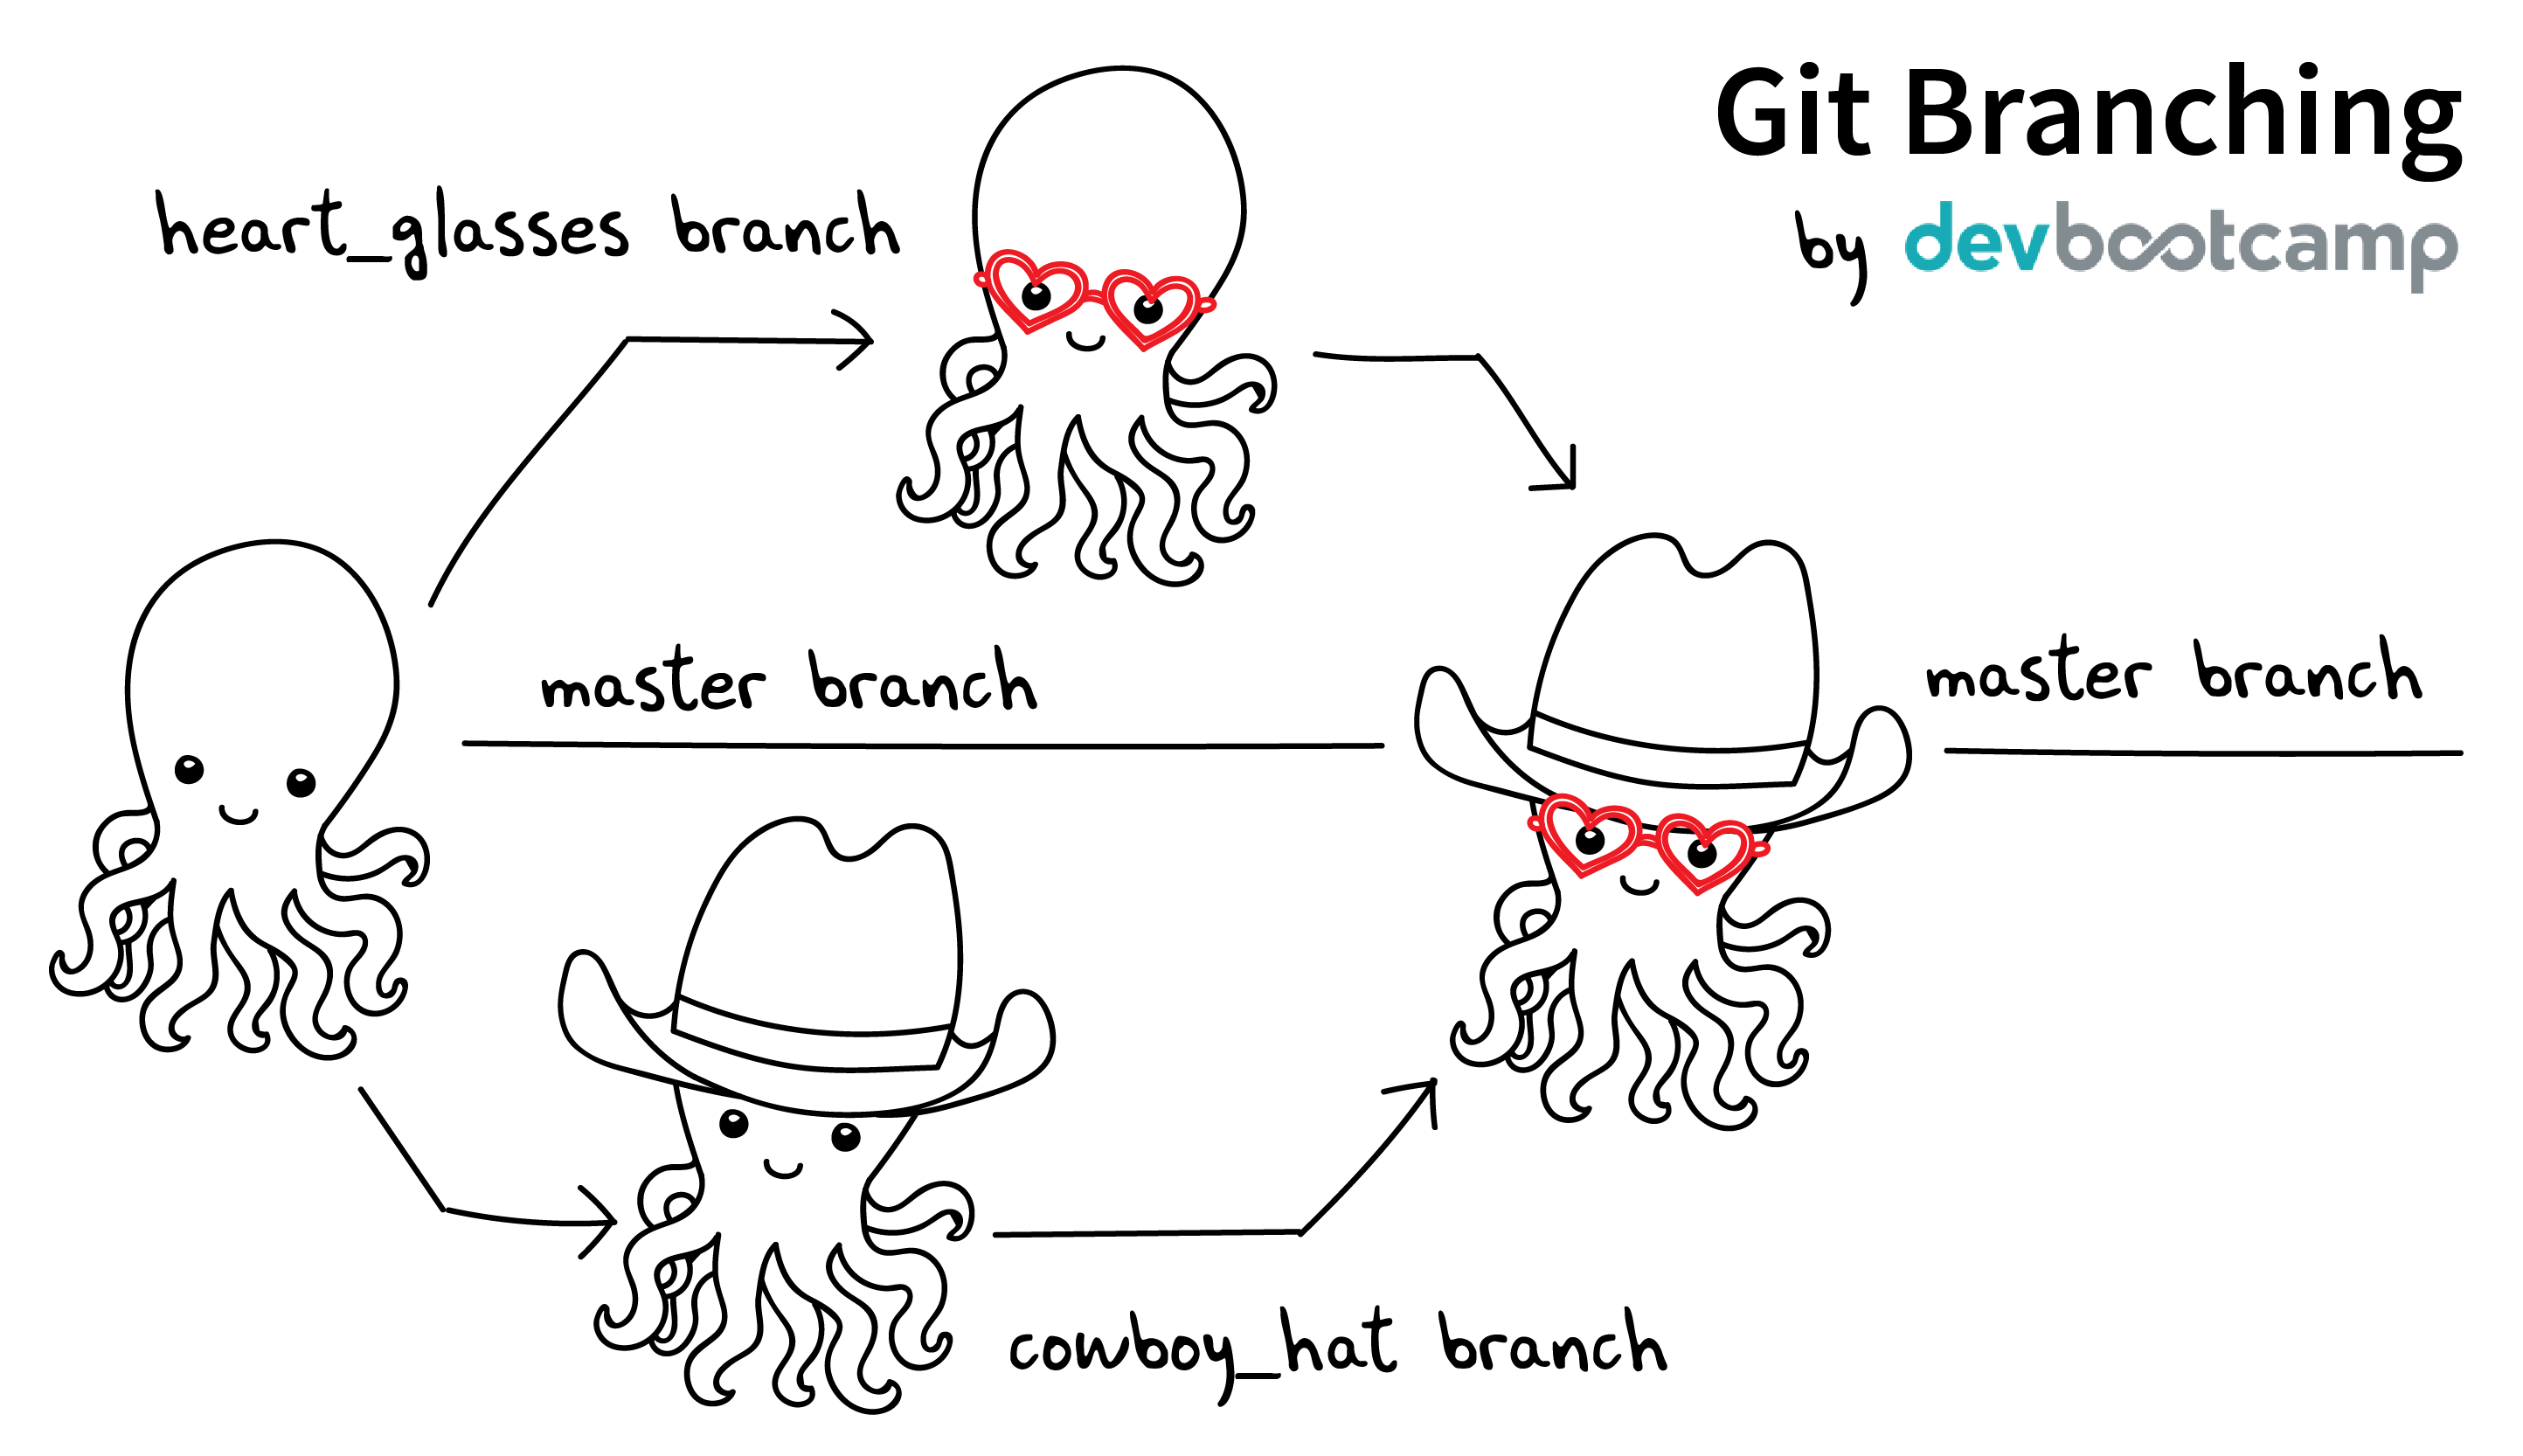
\includegraphics[width=0.9\textwidth]{graphics/git_branching_octopus.png}
\end{frame}

%%%%%%%%%%%%%%%%%%%%%%%%%%%%%%%%%%%%%%%%%%%%%%%%%%

\section{Working together}

\begin{frame}
\frametitle{Working together}
\centering

\includegraphics[width=0.6\textwidth]{graphics/collaboration.png}
\end{frame}

%%%%%%%%%%%%%%%%%%%%%%%%%%%%%%%%%%%%%%%%%%%%%%%%%%

\begin{frame}
\frametitle{Working together}
\begin{itemize}
	\item Git repos can be hosted on a server
	\item $\rightarrow$ other people can access the repo and collaborate
\end{itemize}
\vspace{.5cm}
Services providing such hosting:
\begin{itemize}
	\item GitHub
	\item \textcolor{red}{GitLab} {\footnotesize  $\leftarrow$ what we use in our lab}
	\item Bitbucket
	\item ...
\end{itemize}
\end{frame}

%%%%%%%%%%%%%%%%%%%%%%%%%%%%%%%%%%%%%%%%%%%%%%%%%%

\begin{frame}
\frametitle{GitLab}
\begin{itemize}
	\item create and modify repositories online
	\item admins can manage repos, give access to users...
\end{itemize}
\end{frame}

%%%%%%%%%%%%%%%%%%%%%%%%%%%%%%%%%%%%%%%%%%%%%%%%%%

\begin{frame}
\frametitle{GitLab}
\todo{mini gitlab tut here}
\end{frame}

%%%%%%%%%%%%%%%%%%%%%%%%%%%%%%%%%%%%%%%%%%%%%%%%%%

\begin{frame}
\frametitle{GitLab}
\todo{stuff like git clone, git push, git pull here?}
\end{frame}

%%%%%%%%%%%%%%%%%%%%%%%%%%%%%%%%%%%%%%%%%%%%%%%%%%

\begin{frame}
\frametitle{Change branches}
\end{frame}


\end{document}
